\documentclass{article}


\usepackage{arxiv}
\usepackage{algorithm,algpseudocode}

\usepackage[utf8]{inputenc} % allow utf-8 input
\usepackage[T1]{fontenc}    % use 8-bit T1 fonts
\usepackage{hyperref}       % hyperlinks
\usepackage{url}            % simple URL typesetting
\usepackage{booktabs}       % professional-quality tables
\usepackage{amsfonts}       % blackboard math symbols
\usepackage{nicefrac}       % compact symbols for 1/2, etc.
\usepackage{microtype}      % microtypography
\usepackage{lipsum}
\usepackage{amsmath}
\usepackage{amssymb}
\usepackage{textcomp}
\usepackage[dvipsnames]{xcolor}
\usepackage{graphicx}
\usepackage{subcaption}
\usepackage{bbold}
\usepackage{bm}
\newcommand{\CO}{\mathcal{O}}
\usepackage{wrapfig}
\newcommand\subfig[2]{{Fig.~\ref{#1}{#2}}}
\newcommand\fig[1]{{Fig.~\ref{#1}}}
\usepackage[super]{nth}
\usepackage{dirtytalk}
\usepackage{braket}
%\usepackage{blindtext}
%\usepackage{tcolorbox}
%\usepackage{graphicx}

\usepackage{empheq}
\usepackage[most]{tcolorbox}
\tcbset{highlight math style={boxsep=1mm,colback=blue!30!red!10!white}}

\title{Préparation de Windows 10 pour le TP}


\author{
Pour toute question, veuillez contacter\\
 Juliane U. Klamser\\%\thanks{website}\\
  Gulliver,  ESPCI\\
  Paris \\
  \texttt{Juliane.Klamser@espci.psl.eu} \\
}

\begin{document}
\maketitle

\tableofcontents

%\begin{abstract}
%Bla bla
%\end{abstract}


% keywords can be removed
%\keywords{First keyword \and Second keyword \and More}

\newpage
\section{Remarques générales}
Il existe de nombreux compilateurs C souvent gratuits (même le compilateur de MicroSoft est gratuit), nous vous proposons d'installer GCC le compilateur de GNU parce qu'il existe sur presque toutes les machines et les systèmes d'exploitation. Coder c'est bien, on peut presque tout faire, mais utiliser le travail des autres c'est encore mieux. Au-delà du compilateur, il est très commode de pouvoir bénéficier de très nombreuses librairies que d'autres, beaucoup plus courageux que vous, ont écrites. En fait, ces librairies sont en permanence améliorées et elles dépendent les unes des autres, les recopier et les garder compatibles entre elles est un challenge. 
Heureusement il existe des logiciels qui vous permettent de conserver et d'étendre une chaîne de compilation et de librairies à jour sans trop souffrir. C'est particulièrement vrai sur Linux où ils se nomment \textbf{apt-get}. Sur Windows c'était beaucoup moins simple, mais il existe aujourd'hui de nombreuses solutions qui vous permet de retrouver l’environnement style Linux. Dans ce document, vous trouverez les étapes nécessaires pour installer un sous-système Windows pour Linux (Windows Subsystem for Linux $=$ WSL), qui est une couche de compatibilité permettant d'exécuter des exécutables binaires Linux (au format ELF) de manière native sur Windows 10 et Windows Server 2019.  Au final, vous disposerez, espérons-le, d'un terminal en ligne de commande, appelé terminal Ubuntu.

Le terminal Ubuntu pour Windows possède un grand nombre de caractéristiques que vous trouverez en utilisant le terminal sur Ubuntu :
\begin{itemize}
\item Une gamme inégalée de paquets, de mises à jour et de fonctions de sécurité
\item Bash, Z-Shell, Korn et autres environnements shell sans machines virtuelles ni double amorçage
\item Exécutez des outils natifs tels que SSH, git, apt et dpkg directement depuis votre ordinateur Windows
\item Une vaste communauté d'utilisateurs conviviaux et accessibles
\end{itemize}

\section{Logiciels anti-virus}
Les logiciels anti-virus sont les plus susceptibles de bloquer la préparation de votre ordinateur. Il existe deux scénarios
\begin{enumerate}
\item Vous pouvez désinstaller votre logiciel anti-virus et le réinstaller ultérieurement, une fois que toutes les étapes de préparation sont terminées.
\item Vous ne pouvez pas désinstaller votre logiciel anti-virus.
\end{enumerate}

Comment procéder dans les différents scénarios ?
\begin{enumerate}
\item Dans le premier scénario, désinstallez votre anti-virus et redémarrez votre ordinateur. Après avoir redémarré votre ordinateur, assurez-vous que le logiciel anti-virus n'est plus là.
\item Dans le deuxième scénario:
\begin{enumerate}
\item Si le logiciel anti-virus est Kaspersky: Settings $\rightarrow$ Additional $\rightarrow$ Network $\rightarrow$ Monitored ports: Monitor selected ports only $\rightarrow$ Select $\rightarrow$ Disable the following two: HTTPS  and HTTP with Port 80. 
\begin{figure}[H]
\begin{subfigure}[c]{0.7\textwidth}
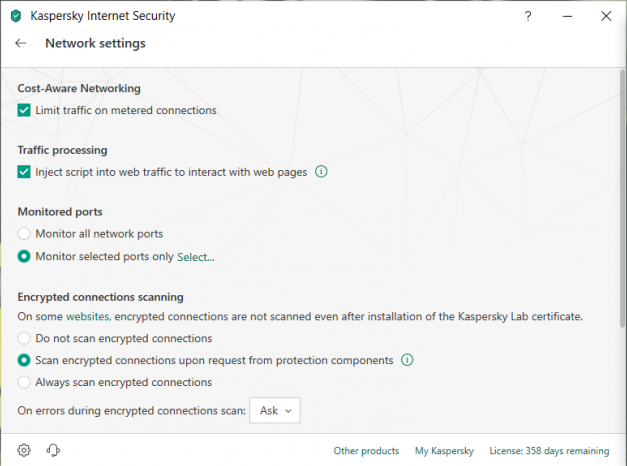
\includegraphics[width=1\textwidth]{Plots/Kasp1.png}
\subcaption{Settings $\rightarrow$ Additional $\rightarrow$ Network $\rightarrow$ Monitored ports: Monitor selected ports only}
\end{subfigure}
\begin{subfigure}[c]{0.3\textwidth}
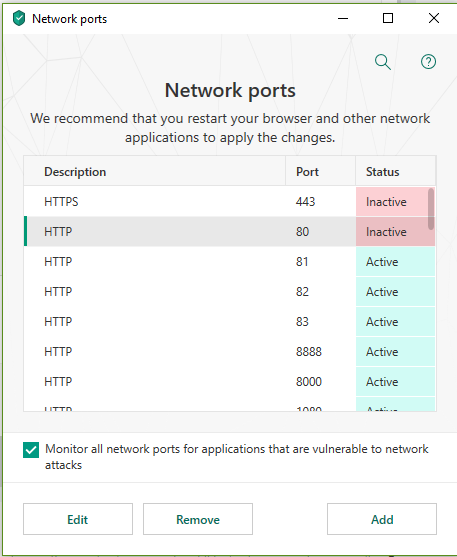
\includegraphics[width=1\textwidth]{Plots/Kasp2.png}
\subcaption{Disable the following two: HTTPS  and HTTP with Port 80}
\end{subfigure}
\caption{Preparation of Kaspersky settings.}
\end{figure}
\item S'il s'agit d'un autre programme anti-virus, nous devrons d'abord essayer sans modifier les paramètres. Si vous êtes bloqué au cours des étapes suivantes, contactez \href{mailto:example@example.com}{juliane.klamser@espci.psl.eu}
\end{enumerate}
\end{enumerate}
\section{Activer la fonction : Windows Subsystem for Linux}
Allez dans le menu Start et recherchez PowerShell. Exécutez-le en tant qu'administrateur :
\begin{figure}[H]
\center
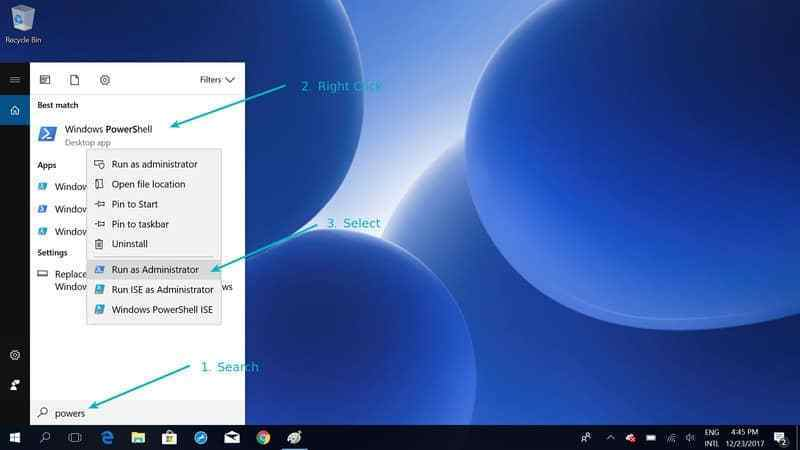
\includegraphics[width=0.8\textwidth]{Plots/Powershell-Ubuntu-install.jpg}
%\caption{Preparation of Kaspersky settings.}
\end{figure}
Après l'ouverture du PowerShell, copiez et passez la ligne suivante dans le terminal PowerShell et appuyez sur ENTER:

\begin{tcolorbox}[width=\textwidth,colback={purple},title={PowerShell terminal},outer arc=0mm,colupper=white]    
    \large\textbf{ Enable-WindowsOptionalFeature -Online -FeatureName Microsoft-Windows-Subsystem-Linux }
\end{tcolorbox}
Il vous sera demandé de confirmer votre choix. Tapez Y ou appuyez sur la touche Entrée :
\begin{figure}[H]
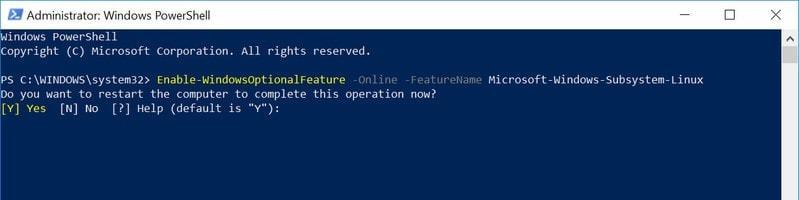
\includegraphics[width=1\textwidth]{Plots/Powershell-Ubuntu-install-2.jpg}
%\caption{Preparation of Kaspersky settings.}
\end{figure}

Maintenant, on devrait vous demander de redémarrer. Même si on ne vous le demande pas, vous devez redémarrer votre système.

\section{Installation de l'application Ubuntu}
Installez une application appelée Ubuntu à partir de l'App Store microsoft (suivez ce lien \href{https://www.microsoft.com/en-us/p/ubuntu/9nblggh4msv6?activetab=pivot:overviewtab}{https://www.microsoft.com/en-us/p/ubuntu/9nblggh4msv6?activetab=pivot:overviewtab}).

Cette application sera votre terminal. 

Ouvrez l'application pour terminer l'installation. 
Il vous sera demandé d'insérer un nom d'utilisateur et d'insérer un mot de passe. 

\textbf{Attention} : Lorsque vous entrez le mot de passe, vous ne verrez rien. Il semble que rien ne se passe. Une fois que vous avez tapé votre mot de passe, appuyez sur ENTER. Il vous sera demandé de confirmer votre mot de passe.

\textbf{Note} : Vous devez noter ce nom d'utilisateur et le mot de passe à un endroit où vous ne le perdez pas. Dans ce document, nous appellerons ce nom d'utilisateur et ce mot de passe Ubuntu-Username et Ubuntu-password.

\section{Installation des paquets nécessaires}
Nous allons ici installer quelques paquets de base pour le terminal ubuntu, dont nous aurons besoin pour le TP, comme par exemple le compilateur. Le compilateur traduit votre code (compréhensible pour un humain) dans un langage qui peut être interprété et exécuté par l'ordinateur. Alors, allons-y.

Tout ce qui suit doit être fait dans votre nouveau terminal ubuntu. Ouvrez l'application. Vous pouvez écrire dans ce terminal. \textbf{Notez que vous ne pouvez vous déplacer entre les lettres qu'avec les touches fléchées de votre clavier. } Si vous utilisez les flèches haut et bas de votre clavier, vous pouvez naviguer entre les commandes que vous avez utilisées dans le passé dans le terminal.

Copiez et collez les commandes suivantes (l'une après l'autre) dans le terminal ubuntu et confirmez avec ENTER. Chaque fois que vous confirmez l'une des commandes suivantes avec ENTER, une installation démarre.  Attendez que l'installation se termine avant de taper la commande suivante. \textbf{Vérifiez attentivement s'il n'y a pas de messages d'erreur après une installation.} En cas de messages d'erreur, contactez \href{mailto:example@example.com}{juliane.klamser@espci.psl.eu}.

\begin{enumerate}
\item commande:
\begin{tcolorbox}[width=\textwidth,colframe=BurntOrange,colback={black},title={ubuntu terminal},outer arc=0mm,colupper=white]  
    \large\textbf{  sudo apt-get update }
\end{tcolorbox}
Vous devrez peut-être entrer votre Ubuntu-password. Vous devrez peut-être confirmer avec "Y". Attendez que l'installation soit terminée. 
Votre résultat devrait être similaire à celui-ci. Il n'y a pas de message de WARNING et pas de message de ERROR.
\begin{figure}[H]
\center
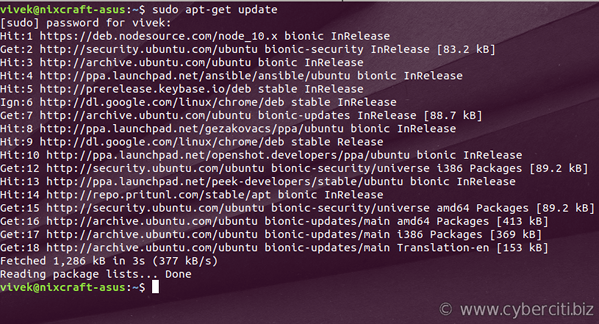
\includegraphics[width=0.7\textwidth]{Plots/What-does-sudo-apt-get-update-command-do-on-Ubuntu-Debian-Linux.png}
%\caption{Preparation of Kaspersky settings.}
\end{figure}
\item commande:
\begin{tcolorbox}[width=\textwidth,colframe=BurntOrange,colback={black},title={ubuntu terminal},outer arc=0mm,colupper=white]  
    \large\textbf{  sudo apt install g++ }
\end{tcolorbox}
Vous devrez peut-être entrer votre Ubuntu-password. Vous devrez peut-être confirmer avec "Y". Attendez que l'installation soit terminée. 
\item commande:
\begin{tcolorbox}[width=\textwidth,colframe=BurntOrange,colback={black},title={ubuntu terminal},outer arc=0mm,colupper=white]  
   \large\textbf{  sudo apt-get install libcairo2-dev }
\end{tcolorbox}
Vous devrez peut-être entrer votre Ubuntu-password. Vous devrez peut-être confirmer avec "Y". Attendez que l'installation soit terminée. 
\item commande:
\begin{tcolorbox}[width=\textwidth,colframe=BurntOrange,colback={black},title={ubuntu terminal},outer arc=0mm,colupper=white]  
    \large\textbf{  sudo apt-get install gnuplot }
\end{tcolorbox}
Vous devrez peut-être entrer votre Ubuntu-password. Vous devrez peut-être confirmer avec "Y". Attendez que l'installation soit terminée. 
\end{enumerate}

\section{Gnuplot}
Gnuplot est un logiciel qui sert à produire des représentations graphiques en deux ou trois dimensions de fonctions numériques ou de données. Il sera très utile pour tracer des données avec quelques lignes. 

Avec la commande sudo apt-get install gnuplot (voir ci-dessus), vous avez déjà installé un gnuplot, que vous pouvez utiliser dans la termina ubuntu. Cependant, si vous préférez une version graphique, ce qui pourrait être plus facile pour le début, vous pouvez télécharger et installer le logiciel à partir de ce site: \href{http://www.gnuplot.info/download.html}{http://www.gnuplot.info/download.html} 

Si possible, choisissez les paramètres par défaut.

\section{Installation d'un éditeur de code}
Vous pouvez choisir l'éditeur de code que vous voulez. 
\subsection{Notepad++}
Une façon simple de commencer et d’utiliser Notepad++. Ce éditeur est léger est assez efficace, d'ici \href{https://notepad-plus-plus.org}{https://notepad-plus-plus.org}. Assurez-vous que vous installez une version compatible avec votre ordinateur.
\begin{figure}[H]
\center
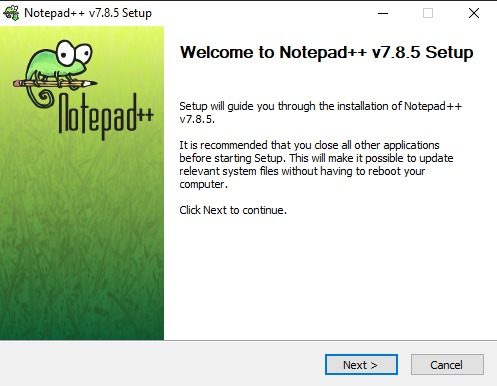
\includegraphics[width=0.4\textwidth]{Plots/Editor_1.jpg}
%\caption{Resultat de pacman -S mingw-w64-x86\_64-pkg-config mingw-w64-x86\_64-gtk3 make}
\end{figure}
\subsection{Visual Studio Code et Atom\label{S:VisCodAtom}}
Vous pouvez essayer atom \href{https://atom.io}{https://atom.io}\\
ou bien Visual Studio Code \href{https://code.visualstudio.com/download}{https://code.visualstudio.com/download}

Les deux éditeurs de code offrent une option qui vous permettent de travailler simultanément sur le même code avec quelqu'un. C'est très utile pour le projet final, lorsque vous travaillez avec un partenaire sur le même code. Cette fonction est appelée "Teletype" pour atom et "live share" pour Visual Studio Code.

\section{Lançons votre premier code C.}
Rendez-vous sur ce site \href{https://github.com/JulianeUta/TP_Programmation2020_ForStudents/blob/master/MyFirstCode.zip}{https://github.com/JulianeUta/TP\_Programmation2020\_ForStudents/blob/master/MyFirstCode.zip} et cliquez sur Download. Un dossier compressé avec votre premier code en C sera téléchargé. L'objectif est de compiler le code et de l'exécuter.
\begin{figure}[H]
\center
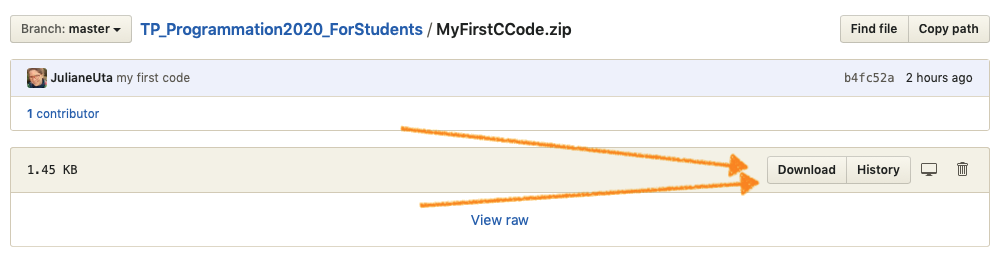
\includegraphics[width=0.6\textwidth]{Plots/FirstCode_1.png}
%\caption{Resultat de pacman -S mingw-w64-x86\_64-pkg-config mingw-w64-x86\_64-gtk3 make}
\end{figure}
Supposons que vous ayez choisi de sauvegarder le dossier compressé dans votre dossier Documents. Ensuite, allez dans votre dossier Documents et faites un clic droit sur le dossier compressé MyFirstCode, puis sélectionnez quelque chose comme "Extraire tout...".
\begin{figure}[H]
\center
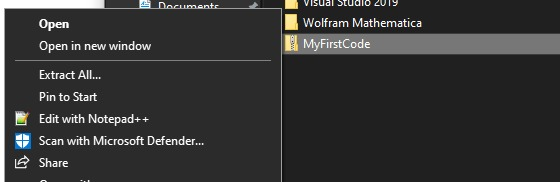
\includegraphics[width=0.6\textwidth]{Plots/FirstCode_2.jpg}
%\caption{Resultat de pacman -S mingw-w64-x86\_64-pkg-config mingw-w64-x86\_64-gtk3 make}
\end{figure}
Il devrait y avoir un dossier normal appelé MyFistCode. Allez dans ce dossier. Il y a peut-être un dossier appelé \_MACOSX.  Vous pouvez supprimer ce dossier \_MACOSX (car ce n'est qu'un artefact de la compression des dossiers sur un ordinateur avec un système d'exploitation différent). Ouvrez le fichier main.c avec Notepad++. C'est votre code. Il devrait ressembler à ceci. 
\begin{figure}[H]
\center
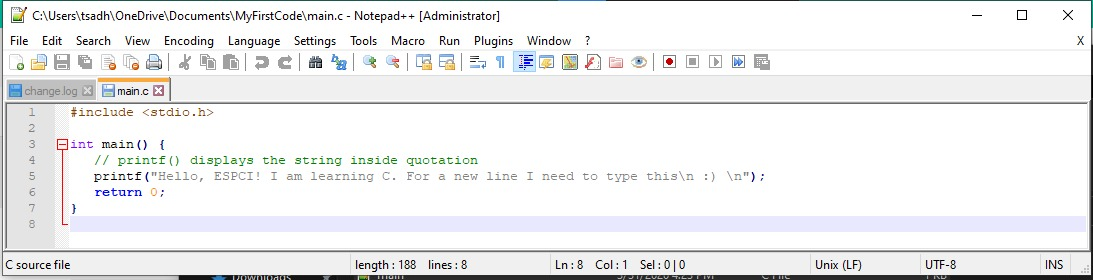
\includegraphics[width=0.95\textwidth]{Plots/FirstCode_9.jpeg}
%\caption{Resultat de pacman -S mingw-w64-x86\_64-pkg-config mingw-w64-x86\_64-gtk3 make}
\end{figure}
Nous voulons maintenant compiler le code (traduire ces mots écrits en quelque chose qui puisse être interprété par l'ordinateur). {\color{Bittersweet}\textbf{Soyez attentifs, car c'est ce que vous ferez de manière extensive pendant ce TP.}}
\subsection{Naviguer dans le terminal jusqu'au dossier du code\label{S:GoToFolder}}
Faites un clic droit sur le dossier MyFirstCode et sélectionnez les propriétés. Nous devons connaître la localisation du dossier avec votre code. Dans l'exemple de la \fig{F:FindFolderAddress}, l'adresse dont nous avons besoin se trouve dans le carré bleu (voir \subfig{F:FindFolderAddress}{b}).
\begin{figure}[H]
\begin{subfigure}[c]{0.5\textwidth}
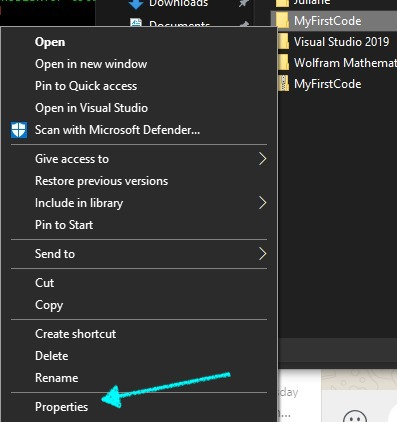
\includegraphics[width=0.75\textwidth]{Plots/FirstCode_3Properties.jpg}
\subcaption{clic droit sur MyFirstCode et sélectionnez les propriétés}
\end{subfigure}
\begin{subfigure}[c]{0.5\textwidth}
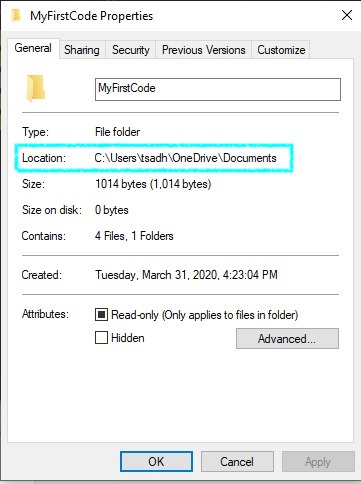
\includegraphics[width=0.75\textwidth]{Plots/FirstCode_4Path.jpg}
\subcaption{Adresse du dossier MyFirstCode}
\end{subfigure}
\caption{Comment trouver l'adresse du dossier.\label{F:FindFolderAddress}}
\end{figure}
Nous utilisons les informations contenues dans le carré bleu et les convertissons en une adresse lisible pour le terminal ubuntu. \\
À noter:
\begin{enumerate}
\item dans le terminal ubuntu \textbf{les noms de dossiers sont séparés par / {\color{Bittersweet}(barre oblique)}} et non par \textbackslash{} (barre oblique inversée).
\item Votre terminal Ubuntu est un système indépendant sur votre ordinateur Windows. Lorsque vous accédez aux dossiers Windows, à partir de votre terminal Ubuntu, vous devez indiquer à Ubuntu qu'il doit regarder sur le système Windows. C'est pourquoi tous les chemins d'accès doivent commencer par /mnt/, ce qui signifie monté.
\end{enumerate}
Maintenant, nous traduisons le chemin indiqué dans le cadre bleu de la \subfig{F:FindFolderAddress}{b} (vous devez adapter votre chemin, avec votre version du cadre bleu). Dans le terminal Ubuntu, le chemin correspondant du dossier MyFirstCode est\\
/mnt/c/Users/tsadhu/OneDrive/Documents/MyFirstCode\\

Nous utilisons maintenant le terminal Ubuntu et naviguons vers ce dossier en tapant
\begin{tcolorbox}[width=\textwidth,colframe=BurntOrange,colback={black},title={ubuntu terminal},outer arc=0mm,colupper=white]  
    \large\textbf{  cd /mnt/c/Users/tsadhu/OneDrive/Documents/MyFirstCode }
\end{tcolorbox}
Si vous tapez maintenant 
%\begin{tcolorbox}[width=\textwidth,colframe=BurntOrange,colback={black},title={ubuntu terminal},outer arc=0mm,colupper=white]
\begin{tcolorbox}[width=\textwidth,colframe=BurntOrange,colback={black},title={ubuntu terminal},outer arc=0mm,colupper=white] 
      \large\textbf{ ls }
\end{tcolorbox}
ce qui signifie qu'il faut \textbf{l}i\textbf{s}ter tous les fichiers de ce dossier (c'est bien un minuscule L et non un I majuscule). Vous devriez voir une sortie comme celle-ci (il y a deux fichiers: Makefile, et main.c).
\begin{figure}[H]
\center
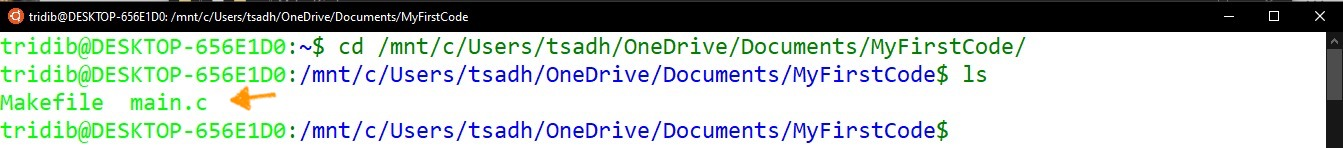
\includegraphics[width=0.9\textwidth]{Plots/FirstCode_5.jpeg}
\end{figure}
\subsection{compiler et exécuter le code}
Pour compiler le code, que vous avez vu dans votre éditeur du code, tapez
\begin{tcolorbox}[width=\textwidth,colframe=BurntOrange,colback={black},title={ubuntu terminal},outer arc=0mm,colupper=white]   
      \large\textbf{  make }
\end{tcolorbox}

Vous devriez voir une sortie comme celle-ci.
\begin{figure}[H]
\center
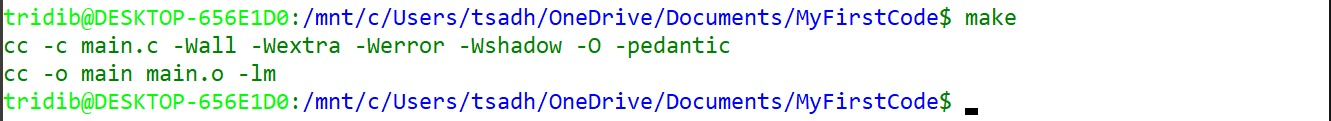
\includegraphics[width=0.9\textwidth]{Plots/FirstCode_6.jpeg}
\end{figure}
Si vous tapez maintenant 
\begin{tcolorbox}[width=\textwidth,colframe=BurntOrange,colback={black},title={ubuntu terminal},outer arc=0mm,colupper=white] 
      \large\textbf{  ls }
\end{tcolorbox}
Vous devriez voir une sortie comme celle-ci. Il existe deux autres fichiers, main.o et main (sans « .o » ou « .c » ). main est écrit dans une langue que l'ordinateur peut interpréter et exécuter. C'est ce que l'on appelle l'exécutable.
 \begin{figure}[H]
\center
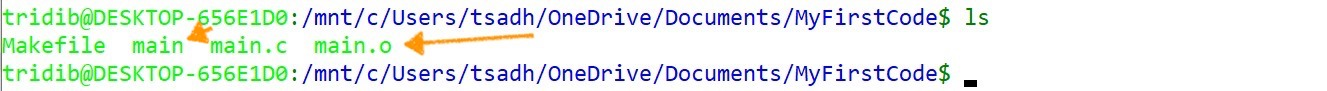
\includegraphics[width=0.9\textwidth]{Plots/FirstCode_7.jpeg}
\end{figure}
Pour exécuter le main, tapez
\begin{tcolorbox}[width=\textwidth,colframe=BurntOrange,colback={black},title={ubuntu terminal},outer arc=0mm,colupper=white]  
      \large\textbf{  ./main }
\end{tcolorbox}
Vous devriez voir une sortie comme celle-ci. 
\begin{figure}[H]
\center
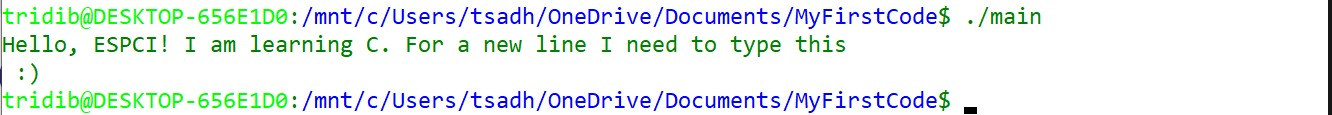
\includegraphics[width=0.9\textwidth]{Plots/FirstCode_8.jpeg}
\end{figure}
Il s'agit de la sortie du code. Si vous voyez ce résultat, alors félicitations à vous. Vous êtes maintenant prêt à commencer le TP.

\section{Installation Xming}
Téléchargez Xming à partir de ce site \href{https://sourceforge.net/projects/xming/}{https://sourceforge.net/projects/xming/}. Démarrez l'installation. Le "Windows defender Firewall" vous demandera les droits d'accès : "ALLOW ACCESS" (AUTORISER L'ACCÈS). Suivez l'installation avec tous les paramètres par défaut (ne changez aucune option).

\section{Test pour le projet final}
Nous devons tester si votre ordinateur est prêt pour le projet final.

Allez à la page suivante et cliquez sur "Download" : \\ \href{https://github.com/JulianeUta/TP_Programmation2020_ForStudents/blob/master/MDFlexBoxRadiusMass.zip}{https://github.com/JulianeUta/TP\_Programmation2020\_ForStudents/blob/master/MDFlexBoxRadiusMass.zip}.

Extrayez le dossier « MDFlexBoxRadiusMass »(clic droit sur le dossier $\rightarrow$ extraire tout). Là encore, vous pouvez supprimer le dossier « \_MACOSX » à l'intérieur du « MDFlexBoxRadiusMass ».

Comme votre code final sera une « animation en temps réel », vous devez indiquer au terminal qu'il doit exporter les données pour les afficher dans une fenêtre graphique. Pour cela, ouvrez le terminal ubuntu et tapez 
\begin{tcolorbox}[width=\textwidth,colframe=BurntOrange,colback={black},title={ubuntu terminal},outer arc=0mm,colupper=white]  
    \large\textbf{  export DISPLAY=:0 }
\end{tcolorbox}
Il devrait ressembler à ceci
\begin{figure}[H]
\center
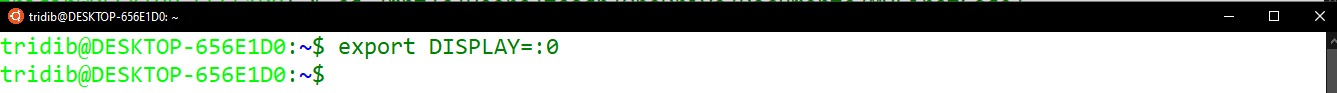
\includegraphics[width=0.9\textwidth]{Plots/MD_1EXPORT.jpeg}
\end{figure}

Maintenant, répétez les étapes décrites au chapitre \ref{S:GoToFolder}, pour naviguer le terminal à l'intérieur du dossier « MDFlexBoxRadiusMass ». Notez que si vous avez déjà utilisé cd /path/to/folder/, vous n'êtes peut-être pas dans le répertoire d'origine. Avec la commande pwd, vous pouvez voir dans quel dossier se trouve le terminal ubuntu en ce moment.
\begin{tcolorbox}[width=\textwidth,colframe=BurntOrange,colback={black},title={ubuntu terminal},outer arc=0mm,colupper=white]  
    \large\textbf{  pwd }
\end{tcolorbox}
Vous devrez peut-être d'abord naviguer vers le dossier d'origine avec la commande
\begin{tcolorbox}[width=\textwidth,colframe=BurntOrange,colback={black},title={ubuntu terminal},outer arc=0mm,colupper=white]  
    \large\textbf{  cd }
\end{tcolorbox}
ou vous pouvez aussi revenir en arrière sur une couche du dossier avec la commande
\begin{tcolorbox}[width=\textwidth,colframe=BurntOrange,colback={black},title={ubuntu terminal},outer arc=0mm,colupper=white]  
    \large\textbf{  cd ..}
\end{tcolorbox}
et ensuite naviguer de là vers l'intérieur du dossier « MDFlexBoxRadiusMass ».

Une fois que vous êtes dans le bon dossier ( « MDFlexBoxRadiusMass »), tapez
\begin{tcolorbox}[width=\textwidth,colframe=BurntOrange,colback={black},title={ubuntu terminal},outer arc=0mm,colupper=white]  
    \large\textbf{  ls }
\end{tcolorbox}
Votre résultat devrait ressembler à ceci
\begin{figure}[H]
\center
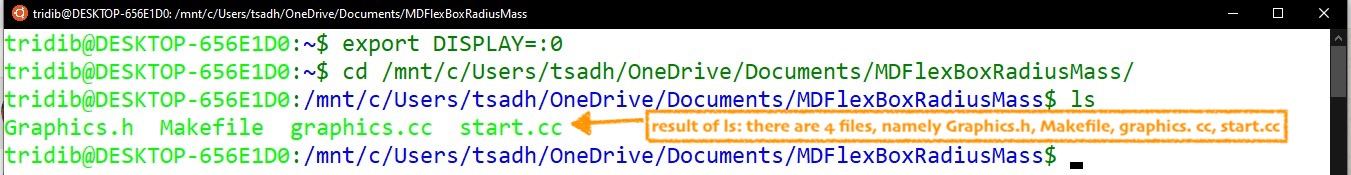
\includegraphics[width=0.9\textwidth]{Plots/MD_2CD.jpeg}
\end{figure}
Maintenant, compilez le code avec
\begin{tcolorbox}[width=\textwidth,colframe=BurntOrange,colback={black},title={ubuntu terminal},outer arc=0mm,colupper=white]  
    \large\textbf{  make }
\end{tcolorbox}
et listez à nouveau tous les fichiers avec
\begin{tcolorbox}[width=\textwidth,colframe=BurntOrange,colback={black},title={ubuntu terminal},outer arc=0mm,colupper=white]  
    \large\textbf{  ls }
\end{tcolorbox}
vous devriez voir 3 autres fichiers (graphics.o, start.o, et start) comme ici
\begin{figure}[H]
\center
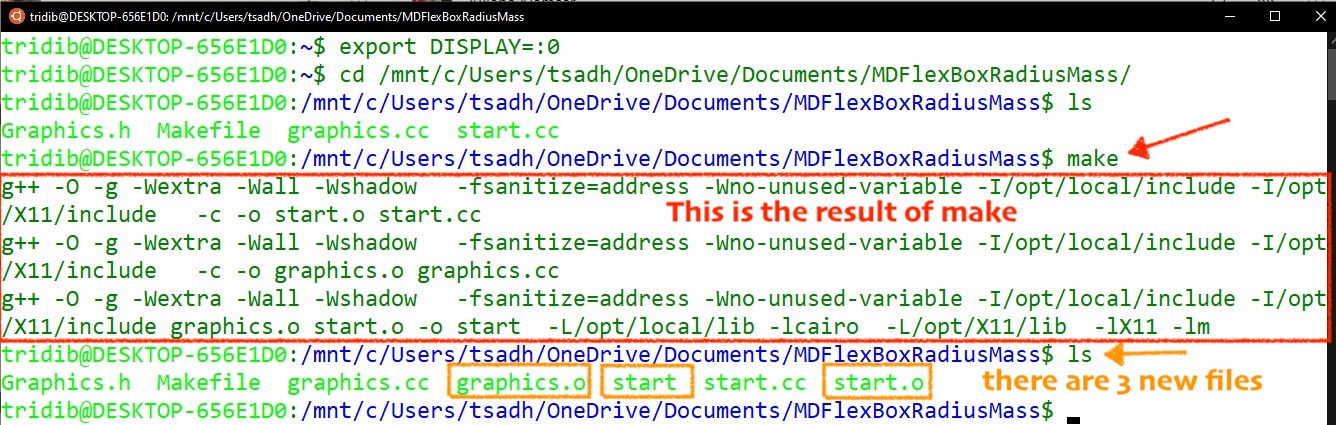
\includegraphics[width=0.9\textwidth]{Plots/MD_3Make.jpeg}
\end{figure}
Dans ce cas, l'exécutable est appelé start. Nous lançons l'exécutable avec la commande suivante
\begin{tcolorbox}[width=\textwidth,colframe=BurntOrange,colback={black},title={ubuntu terminal},outer arc=0mm,colupper=white]  
    \large\textbf{  ./start }
\end{tcolorbox}
Une fenêtre Xming devrait s'ouvrir comme ici
\begin{figure}[H]
\center
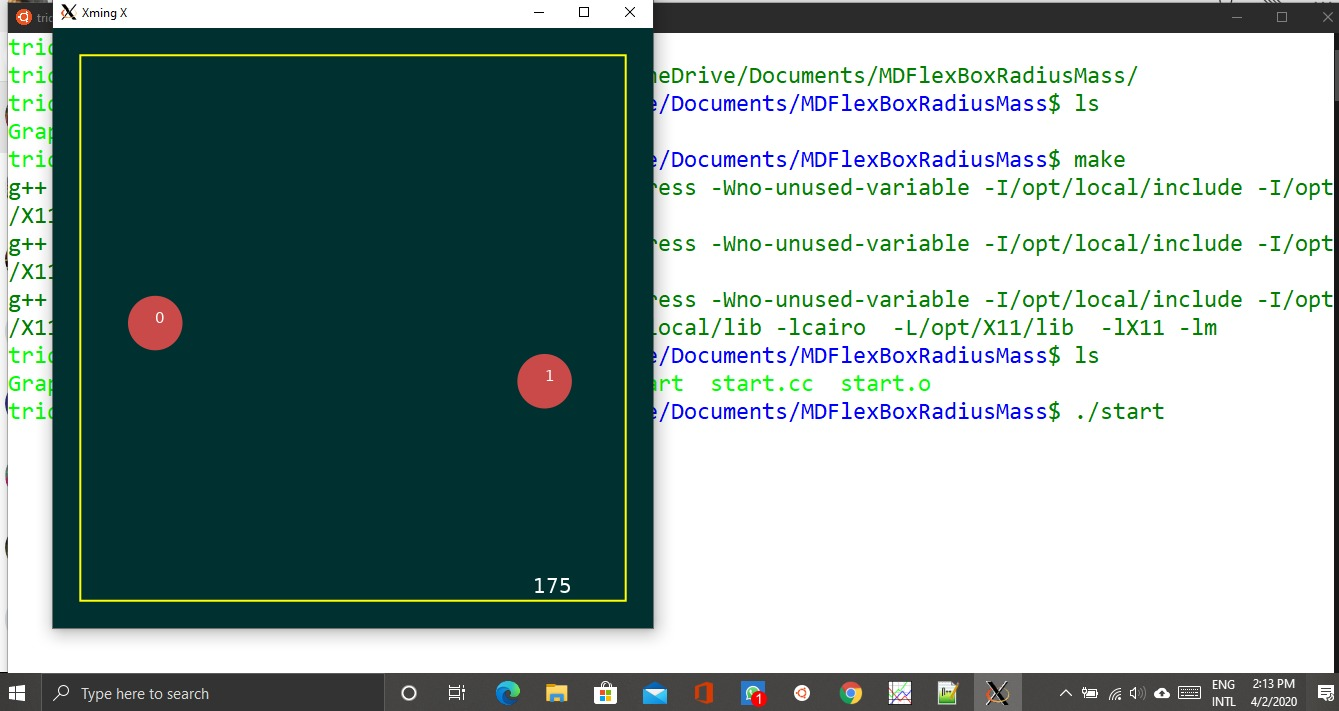
\includegraphics[width=0.9\textwidth]{Plots/MD_4XMing.jpeg}
\end{figure}
Vous devriez voir un carré vert avec deux particules rouges à l'intérieur et un petit compteur blanc en bas à droite qui augmente.

Si la fenêtre XMing ne s'ouvre pas : allez à START, cherchez l'application XMing et ouvrez l'application. Retournez au terminal ubuntu, appuyez sur les touches ctrl + c et tapez à nouveau
\begin{tcolorbox}[width=\textwidth,colframe=BurntOrange,colback={black},title={ubuntu terminal},outer arc=0mm,colupper=white]  
    \large\textbf{./start}
\end{tcolorbox}
Si vous ne voyez pas la fenêtre Xming avec les deux cercles rouges, contactez \href{mailto:example@example.com}{juliane.klamser@espci.psl.eu}.
\subsection{Comment travailler simultanément avec quelqu'un d'autre sur le même code ?}
Comme mentionné au chapitre \ref{S:VisCodAtom}, vous pouvez utiliser les fonctions intégrées des éditeurs de code Visual Studio Code ou Atom. 

Une autre méthode professionnelle, qu'il convient de mentionner, est GitHub. Elle est très puissante et largement utilisée. Cependant, elle nécessite une certaine formation.

La méthode la plus simple est de créer un compte dropbox et d'utiliser dropbox paper. Si vous copiez votre code dans le fichier du dropbox paper, vous et votre partenaire pouvez travailler sur le même code en même temps.



%\bibliographystyle{unsrt}  
%\bibliography{references}  %%% Remove comment to use the external .bib file (using bibtex).
%%% and comment out the ``thebibliography'' section.

\end{document}
